This chapter provides detailed specifications of the system under development.

\section{Functional Requirements}

This section describes each function/feature provided by our system. These functions are logically grouped into modules based on their purpose/users/mode of operations etc (as per our system). A functional hierarchy may look like:
\begin{outline}
  \1 Module 1:
  \2 Function 1:
  \2 Function 2:
  \3 Sub Function 1
  \3 Sub Function 2
  \1 Module 2:
  \2 Function 1:
  \2 Function 2:
  \1 .........
\end{outline}

% --- The above is to be modified as per your project, e.g. a flat list if your system has limited functional requirements.

\section{Non-functional Requirements}

\subsection{Performance Requirement}

\begin{itemize}
    \item The specification of the computer on which our system is hosted need to be extremely high because thousands of users might use the portal at the same time. Therefore, high performance of the computer on which the server is hosted is needed.
    
    \item Fetching the dashboard to view information and recommended outfits shall take no longer than 5 seconds to load the page.
\end{itemize}

\subsection{Safety Requirement}
\begin{itemize}
    \item The system must not halt or lag, especially during the update time and must not go down under high traffic. In order to ensure safety of the server, it is suggested that it is hosted on two computers - one kept as a backup.
    
    \item The system is harmless and would  not case harm to any human being.
\end{itemize}

\subsection{Security Requirement}
\begin{itemize}
    \item It must be ensured that only the authorized admins, with valid user credentials, have access to the data of the users in order to ensure user privacy. 
    
    \item The system will use databases from authentic sources and fashion stores.
    
    \item Any user other than the system admin can only view the information but can in no  way modify it except their personal information and their cart details.
    
    \item System has different two different types of users and both of them have constrained access. 
\end{itemize}

\subsection{User Documentation}
\begin{itemize}
    \item A user will not be provided with the manual as such but would be given some tutorials about how to use the website which would be available on the web portal. 
\end{itemize}

\subsection{Error Handling}
\begin{itemize}
    \item The system prevents data loss by carefully handling all expected and non-expected errors. 
\end{itemize}

\section{External Interfaces}

\subsection{User Interfaces}

\subsubsection{Customer Interface}

\begin{outline}
  \1 Homepage
  
  This interface would be visible to all the users and would lead to multiple other interfaces such as Profile, Login, etc. 
  
  \1 Login
  
  This interface enables user to log into the system using valid credentials, and redirects him/her to the homepage in the credentials are validated, otherwise an error message is displayed. Login interface requires 'User Name' and 'Password' as the mandatory fields. 
  
  \1 Registration:
  
  This page allows a new user to create an account by filling the mandatory fields of 'User Name', 'Email', 'Password' and 'Confirmed Password'. In case of valid details, login becomes possible for the user, else he is redirected to the same Registration page.
  
  \1 Profile
  
  A user would be able to see this interface if they have created an account and are logged into the system. This interface would enable them to view their account details and their previously searched/recommended outfit statistics.
  
  \1 Cart
  
  This interface enables a user to view their selected recommended outfits and would show them the third-party referral links to each of their chosen outfits. 
  
 \end{outline}
 \subsubsection{System Admin Interface}
 \begin{outline}
   \1 Login
   
   Using the login interface, the system admin would log into the system using his/her valid credentials and would be redirected to the system admin homepage
   
   \1 Homepage
   
   This interface enables the system admin to get redirected to multiple other navigation pages such as User Details, and Vendor details.
   
   \1 User Details
   
   This interface contains user details such as their personal information, their cart details and their preferred trend statistics.
   
   \1 Vendor Details
   
   This interface allows the system admin to view details of the vendor such as the trends of their most recommended outfits, new additions to their outfit database, top users visiting the respective vendor page (using the referral link.
   
 \end{outline}

\subsection{User Interfaces}
This section includes our mockup screens and briefly explains them.

\subsection{Application Program Interface (API)}
This section describes the library or API interface to our system.

\subsection{Hardware/Communication Interfaces}
This section describes our project's specific hardware/network interfaces.

\section{Use Cases}
This section presents detailed use cases of our system.

\section{Datasets}
This section describes the specific dataset(s) used to build our system. An appropriate snapshot of the dataset(s) is also included. Futher details, when needed, are presented in the appendix.

\section{System Diagram}
The following diagrams gives an overview of different modules of our system.

\begin{figure}[ht]
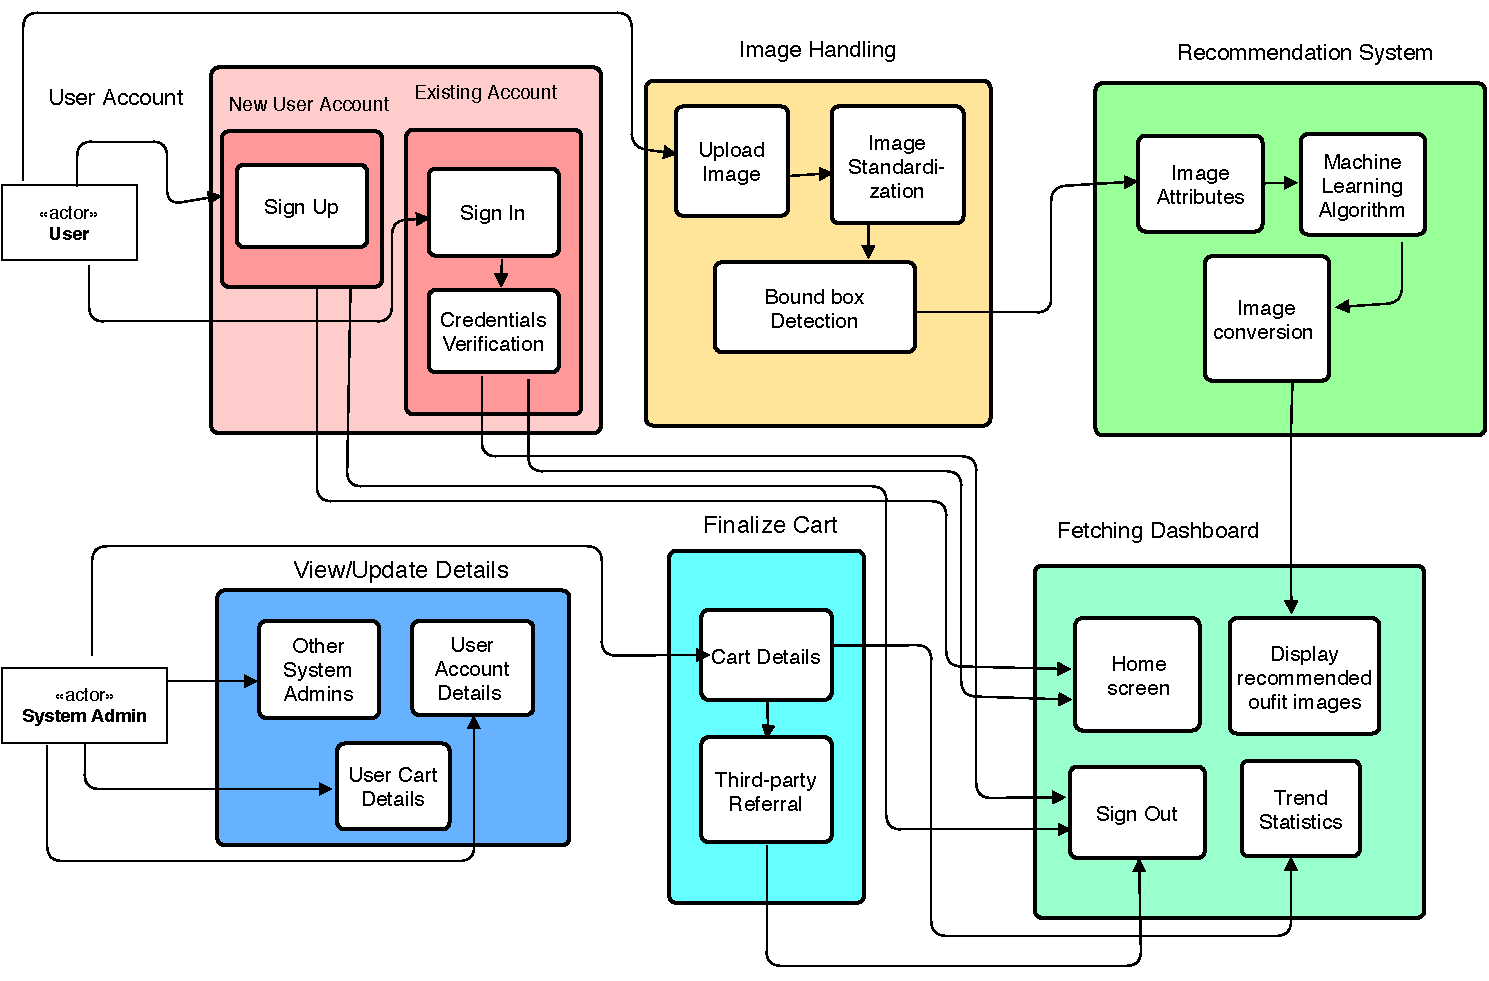
\includegraphics[width=15cm]{images/systemDiagram.pdf} 
\centering
\caption{Module-wise System Diagram}
\end{figure}

\section{Data Flow Diagram}
Rudimentary data flow diagrams for the system have also been constructed, given below:

\begin{figure}[ht]
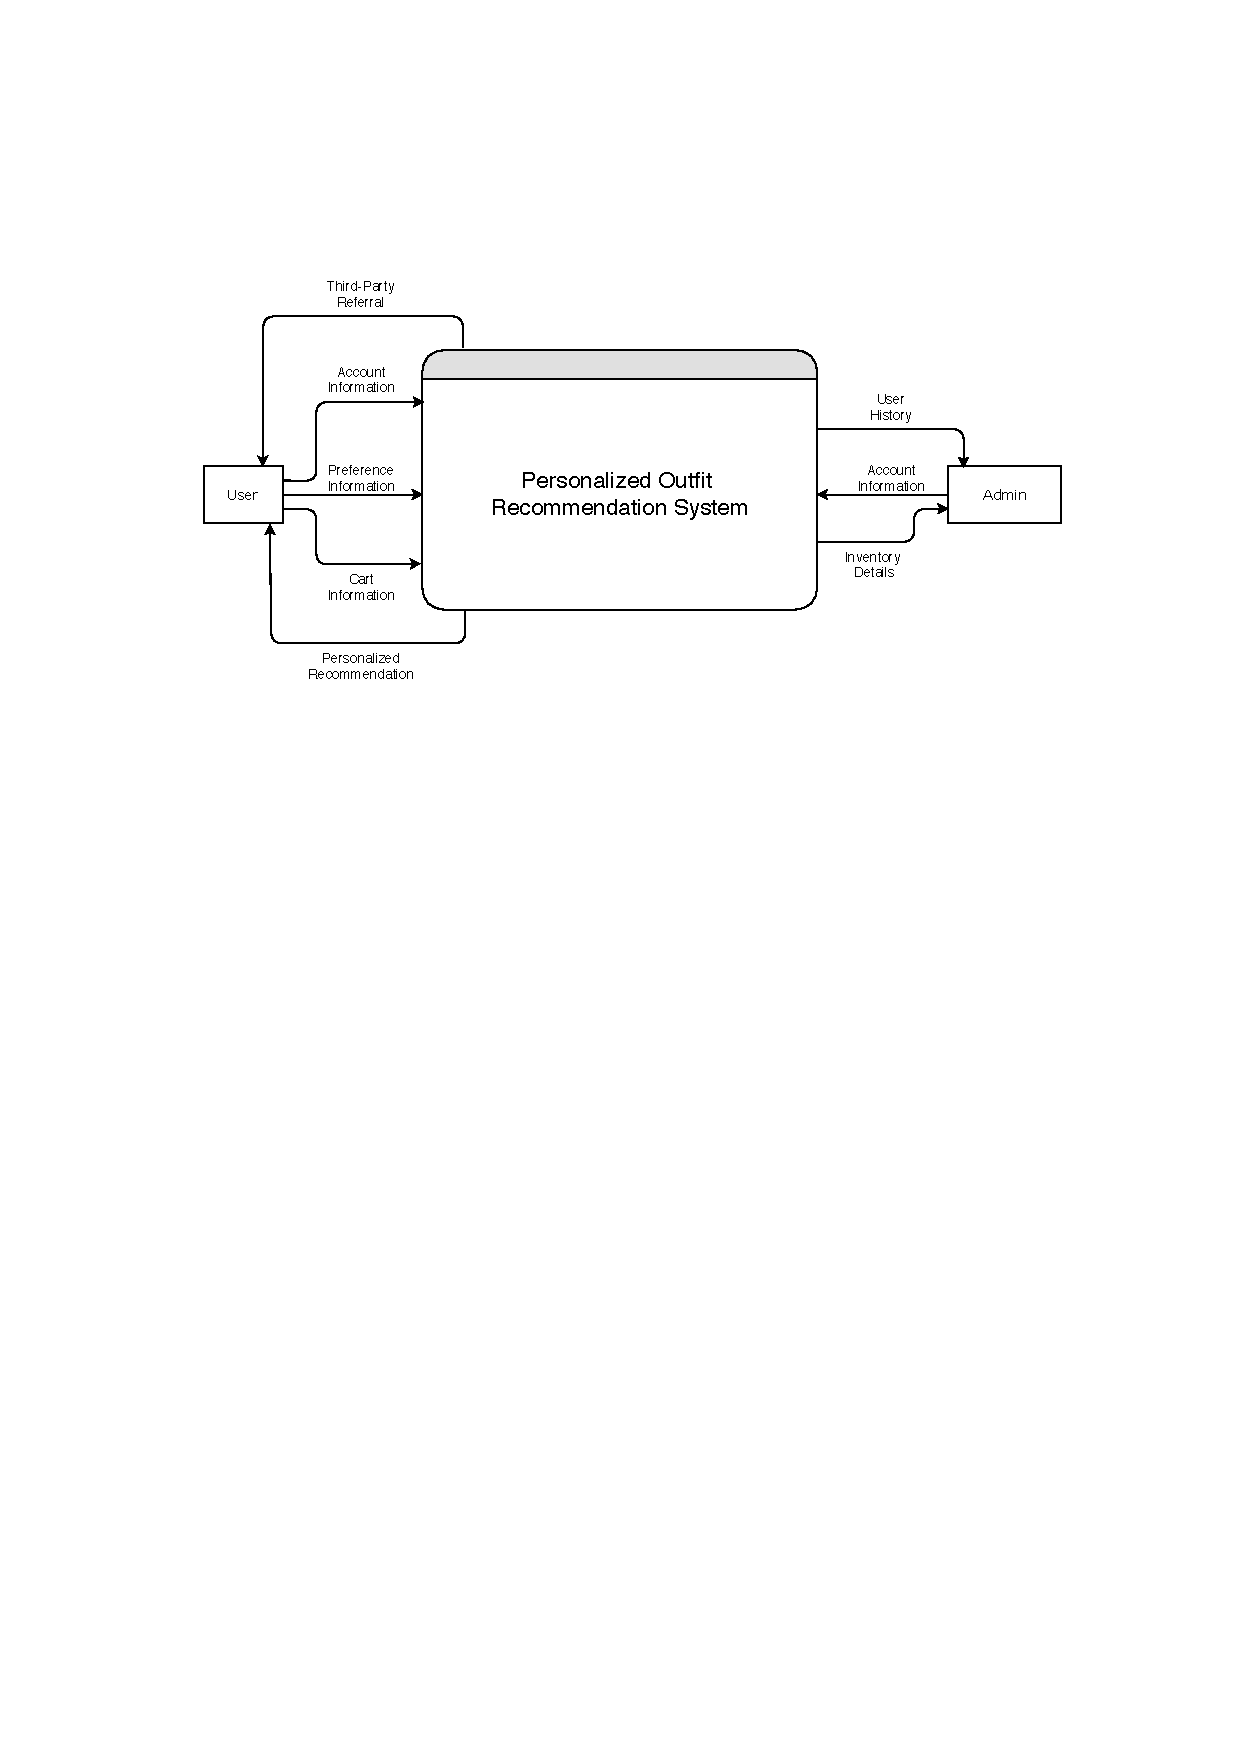
\includegraphics[width=15cm]{images/dfdContext.pdf} 
\centering
\caption{Context Level DFD}
\end{figure}

\begin{figure}[ht]
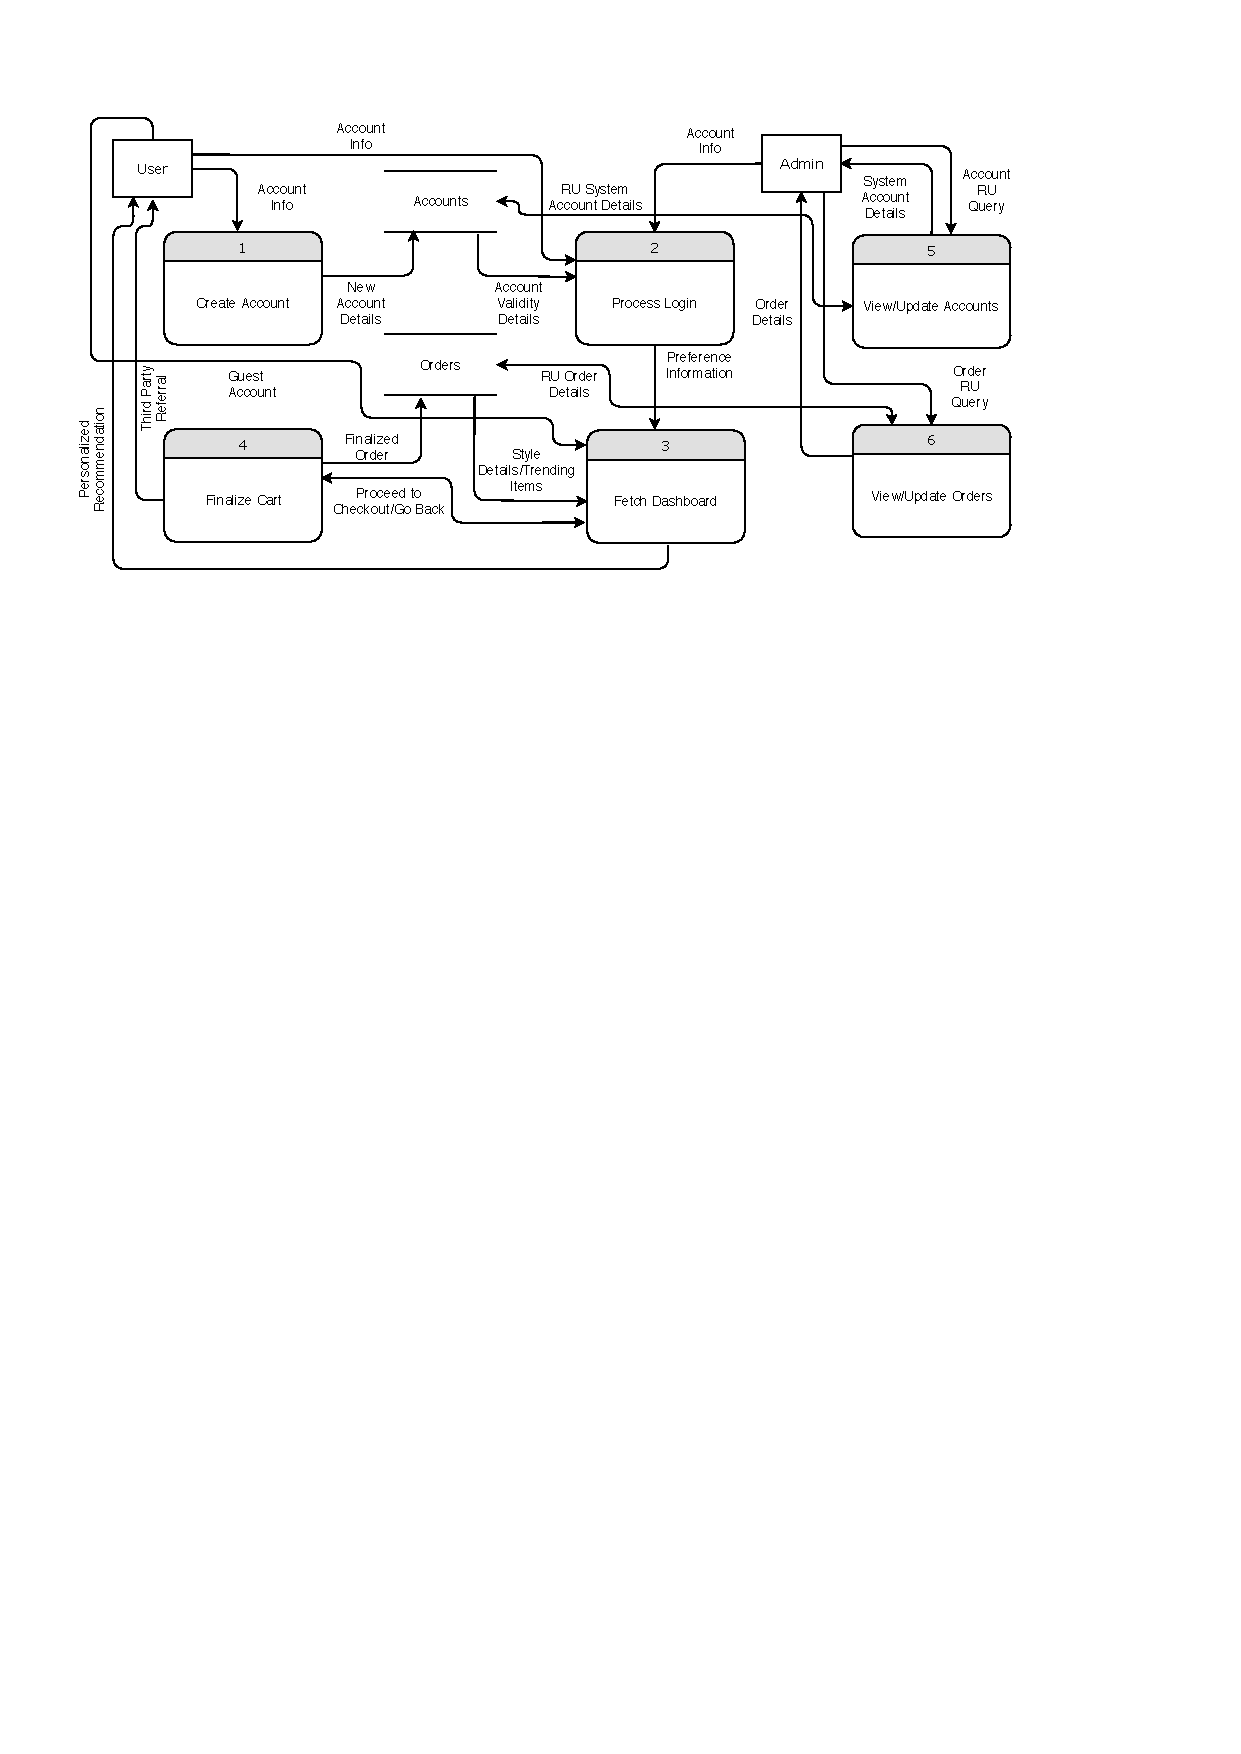
\includegraphics[width=15cm]{images/dfd0.pdf} 
\centering
\caption{0-Level DFD}
\end{figure}
